% Options for packages loaded elsewhere
\PassOptionsToPackage{unicode}{hyperref}
\PassOptionsToPackage{hyphens}{url}
%
\documentclass[
  man,floatsintext]{apa6}
\usepackage{amsmath,amssymb}
\usepackage{lmodern}
\usepackage{iftex}
\ifPDFTeX
  \usepackage[T1]{fontenc}
  \usepackage[utf8]{inputenc}
  \usepackage{textcomp} % provide euro and other symbols
\else % if luatex or xetex
  \usepackage{unicode-math}
  \defaultfontfeatures{Scale=MatchLowercase}
  \defaultfontfeatures[\rmfamily]{Ligatures=TeX,Scale=1}
\fi
% Use upquote if available, for straight quotes in verbatim environments
\IfFileExists{upquote.sty}{\usepackage{upquote}}{}
\IfFileExists{microtype.sty}{% use microtype if available
  \usepackage[]{microtype}
  \UseMicrotypeSet[protrusion]{basicmath} % disable protrusion for tt fonts
}{}
\makeatletter
\@ifundefined{KOMAClassName}{% if non-KOMA class
  \IfFileExists{parskip.sty}{%
    \usepackage{parskip}
  }{% else
    \setlength{\parindent}{0pt}
    \setlength{\parskip}{6pt plus 2pt minus 1pt}}
}{% if KOMA class
  \KOMAoptions{parskip=half}}
\makeatother
\usepackage{xcolor}
\IfFileExists{xurl.sty}{\usepackage{xurl}}{} % add URL line breaks if available
\IfFileExists{bookmark.sty}{\usepackage{bookmark}}{\usepackage{hyperref}}
\hypersetup{
  pdftitle={Satisfying housework division? Gender role beliefs and religion as moderators of housework division and satisfaction},
  pdfauthor={Carlotta Reinhardt1, Margaret Bassney1, \& Anushree Goswami1},
  pdflang={en-EN},
  hidelinks,
  pdfcreator={LaTeX via pandoc}}
\urlstyle{same} % disable monospaced font for URLs
\usepackage{longtable,booktabs,array}
\usepackage{calc} % for calculating minipage widths
% Correct order of tables after \paragraph or \subparagraph
\usepackage{etoolbox}
\makeatletter
\patchcmd\longtable{\par}{\if@noskipsec\mbox{}\fi\par}{}{}
\makeatother
% Allow footnotes in longtable head/foot
\IfFileExists{footnotehyper.sty}{\usepackage{footnotehyper}}{\usepackage{footnote}}
\makesavenoteenv{longtable}
\usepackage{graphicx}
\makeatletter
\def\maxwidth{\ifdim\Gin@nat@width>\linewidth\linewidth\else\Gin@nat@width\fi}
\def\maxheight{\ifdim\Gin@nat@height>\textheight\textheight\else\Gin@nat@height\fi}
\makeatother
% Scale images if necessary, so that they will not overflow the page
% margins by default, and it is still possible to overwrite the defaults
% using explicit options in \includegraphics[width, height, ...]{}
\setkeys{Gin}{width=\maxwidth,height=\maxheight,keepaspectratio}
% Set default figure placement to htbp
\makeatletter
\def\fps@figure{htbp}
\makeatother
\setlength{\emergencystretch}{3em} % prevent overfull lines
\providecommand{\tightlist}{%
  \setlength{\itemsep}{0pt}\setlength{\parskip}{0pt}}
\setcounter{secnumdepth}{-\maxdimen} % remove section numbering
% Make \paragraph and \subparagraph free-standing
\ifx\paragraph\undefined\else
  \let\oldparagraph\paragraph
  \renewcommand{\paragraph}[1]{\oldparagraph{#1}\mbox{}}
\fi
\ifx\subparagraph\undefined\else
  \let\oldsubparagraph\subparagraph
  \renewcommand{\subparagraph}[1]{\oldsubparagraph{#1}\mbox{}}
\fi
\ifLuaTeX
\usepackage[bidi=basic]{babel}
\else
\usepackage[bidi=default]{babel}
\fi
\babelprovide[main,import]{english}
% get rid of language-specific shorthands (see #6817):
\let\LanguageShortHands\languageshorthands
\def\languageshorthands#1{}
% Manuscript styling
\usepackage{upgreek}
\captionsetup{font=singlespacing,justification=justified}

% Table formatting
\usepackage{longtable}
\usepackage{lscape}
% \usepackage[counterclockwise]{rotating}   % Landscape page setup for large tables
\usepackage{multirow}		% Table styling
\usepackage{tabularx}		% Control Column width
\usepackage[flushleft]{threeparttable}	% Allows for three part tables with a specified notes section
\usepackage{threeparttablex}            % Lets threeparttable work with longtable

% Create new environments so endfloat can handle them
% \newenvironment{ltable}
%   {\begin{landscape}\centering\begin{threeparttable}}
%   {\end{threeparttable}\end{landscape}}
\newenvironment{lltable}{\begin{landscape}\centering\begin{ThreePartTable}}{\end{ThreePartTable}\end{landscape}}

% Enables adjusting longtable caption width to table width
% Solution found at http://golatex.de/longtable-mit-caption-so-breit-wie-die-tabelle-t15767.html
\makeatletter
\newcommand\LastLTentrywidth{1em}
\newlength\longtablewidth
\setlength{\longtablewidth}{1in}
\newcommand{\getlongtablewidth}{\begingroup \ifcsname LT@\roman{LT@tables}\endcsname \global\longtablewidth=0pt \renewcommand{\LT@entry}[2]{\global\advance\longtablewidth by ##2\relax\gdef\LastLTentrywidth{##2}}\@nameuse{LT@\roman{LT@tables}} \fi \endgroup}

% \setlength{\parindent}{0.5in}
% \setlength{\parskip}{0pt plus 0pt minus 0pt}

% Overwrite redefinition of paragraph and subparagraph by the default LaTeX template
% See https://github.com/crsh/papaja/issues/292
\makeatletter
\renewcommand{\paragraph}{\@startsection{paragraph}{4}{\parindent}%
  {0\baselineskip \@plus 0.2ex \@minus 0.2ex}%
  {-1em}%
  {\normalfont\normalsize\bfseries\itshape\typesectitle}}

\renewcommand{\subparagraph}[1]{\@startsection{subparagraph}{5}{1em}%
  {0\baselineskip \@plus 0.2ex \@minus 0.2ex}%
  {-\z@\relax}%
  {\normalfont\normalsize\itshape\hspace{\parindent}{#1}\textit{\addperi}}{\relax}}
\makeatother

% \usepackage{etoolbox}
\makeatletter
\patchcmd{\HyOrg@maketitle}
  {\section{\normalfont\normalsize\abstractname}}
  {\section*{\normalfont\normalsize\abstractname}}
  {}{\typeout{Failed to patch abstract.}}
\patchcmd{\HyOrg@maketitle}
  {\section{\protect\normalfont{\@title}}}
  {\section*{\protect\normalfont{\@title}}}
  {}{\typeout{Failed to patch title.}}
\makeatother

\usepackage{xpatch}
\makeatletter
\xapptocmd\appendix
  {\xapptocmd\section
    {\addcontentsline{toc}{section}{\appendixname\ifoneappendix\else~\theappendix\fi\\: #1}}
    {}{\InnerPatchFailed}%
  }
{}{\PatchFailed}
\usepackage{lineno}

\linenumbers
\usepackage{csquotes}
\usepackage[titles]{tocloft}
\cftpagenumbersoff{figure}
\renewcommand{\cftfigpresnum}{\itshape\figurename\enspace}
\renewcommand{\cftfigaftersnum}{.\space}
\setlength{\cftfigindent}{0pt}
\setlength{\cftafterloftitleskip}{0pt}
\settowidth{\cftfignumwidth}{Figure 10.\qquad}
\cftpagenumbersoff{table}
\renewcommand{\cfttabpresnum}{\itshape\tablename\enspace}
\renewcommand{\cfttabaftersnum}{.\space}
\setlength{\cfttabindent}{0pt}
\setlength{\cftafterloftitleskip}{0pt}
\settowidth{\cfttabnumwidth}{Table 10.\qquad}
\ifLuaTeX
  \usepackage{selnolig}  % disable illegal ligatures
\fi

\title{Satisfying housework division? Gender role beliefs and religion as moderators of housework division and satisfaction}
\author{Carlotta Reinhardt\textsuperscript{1}, Margaret Bassney\textsuperscript{1}, \& Anushree Goswami\textsuperscript{1}}
\date{}


\shorttitle{gender roles, housework and satisfaction}

\affiliation{\vspace{0.5cm}\textsuperscript{1} Smith College}

\begin{document}
\maketitle

\hypertarget{results}{%
\section{Results}\label{results}}

\hypertarget{analysis-strategy}{%
\subsection{Analysis Strategy}\label{analysis-strategy}}

To test our hypotheses that gender role beliefs and religion moderate the relationship between housework distribution and satisfaction, we used multilevel modeling and the Actor-Partner Interdependence Model (APIM; Kenny, Kashy, \& Cook, 2006). The APIM measures the effect of the explanatory variables for both members in a dyad at the same time, so actor as well as partner effects could be considered in our analysis. This way, it is possible to see how one partner's housework distribution effects both their own satisfaction with the housework distribution (actor effect) and their partner's satisfaction with the housework distribution (partner effect). In this analysis, we will further look at the moderating effect of each partner's gender role beliefs on the two actor effects (shown in figure 1) as well as on the partner effects. (THIS FOLLOWING SENTENCE CONFUSES ME!) The APIM measures proportion of variance in satisfaction that occurs between dyads vs.~the total variation present. In other words, the model considers how much of the variation in satisfaction is caused by the dyad. This allows to estimate satisfaction with the distribution of housework as a function of both housework distribution and the the random errors at both the individual and dyad level. This accounts for the non-independent data.



\begin{figure}
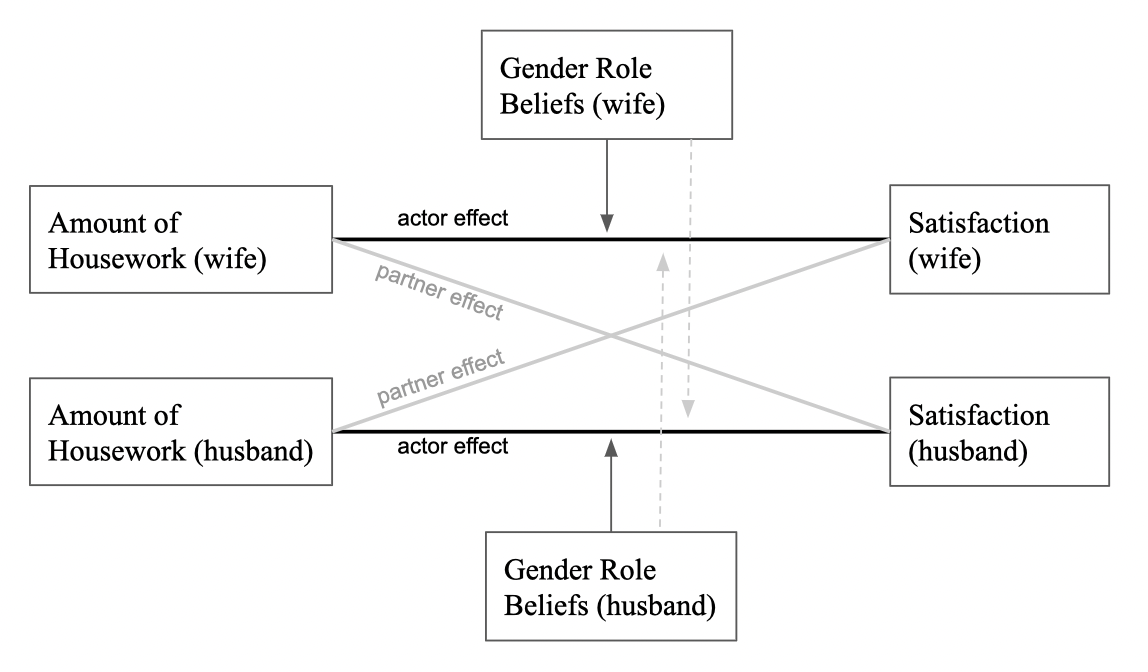
\includegraphics[width=3.83in]{APIM} \caption{Actor Partner Effects in the APIM.}\label{fig:unnamed-chunk-3}
\end{figure}

\hypertarget{main-results}{%
\subsection{Main Results}\label{main-results}}

\hypertarget{gender-role-beliefs-as-a-mediator}{%
\subsubsection{Gender Role Beliefs as a mediator}\label{gender-role-beliefs-as-a-mediator}}

The summary table above is just of the actor partner effects with no moderation. The only relationship that is statistically significant is the one between the wife's satisfaction level and her average housework. We know this because the p-value for \texttt{as.factor(genderE\_A)1:Cavg\_housework\_female\_A} is 0.0041, which is less than 0.05. Since the value for this relationship is -0.029132, it signifies that as the wife's average housework increases, her satisfaction level decreases.

as.factor(genderE\_A)0:Cavg\_housework\_female\_A:Cavg\_grbs\_P = For men, keeping their average female-typed housework tasks constant, for every one unit increase in avg grbs, their housework satisfaction increases by 0.02.

For women, gender role beliefs significantly moderated the relationship between her own housework distribution and her satisfaction with the housework distribution. The moderation effect was 0.07 (\emph{p} = 0.00, \emph{se} = 0.02). For every one unit increase in her gender role beliefs, her satisfaction increases by 0.07 while keeping housework distribution constant. Again for women, her partners gender role beliefs significantly moderated the relationship between her own housework distribution and her satisfaction with the housework distribution. The moderation effect was -0.06 (\emph{p} = 0.01,se = 0.02). For every one unit increase in her partners gender role beliefs, her own satisfaction increased by -0.06 while keeping housework distribution constant.



\begin{figure}
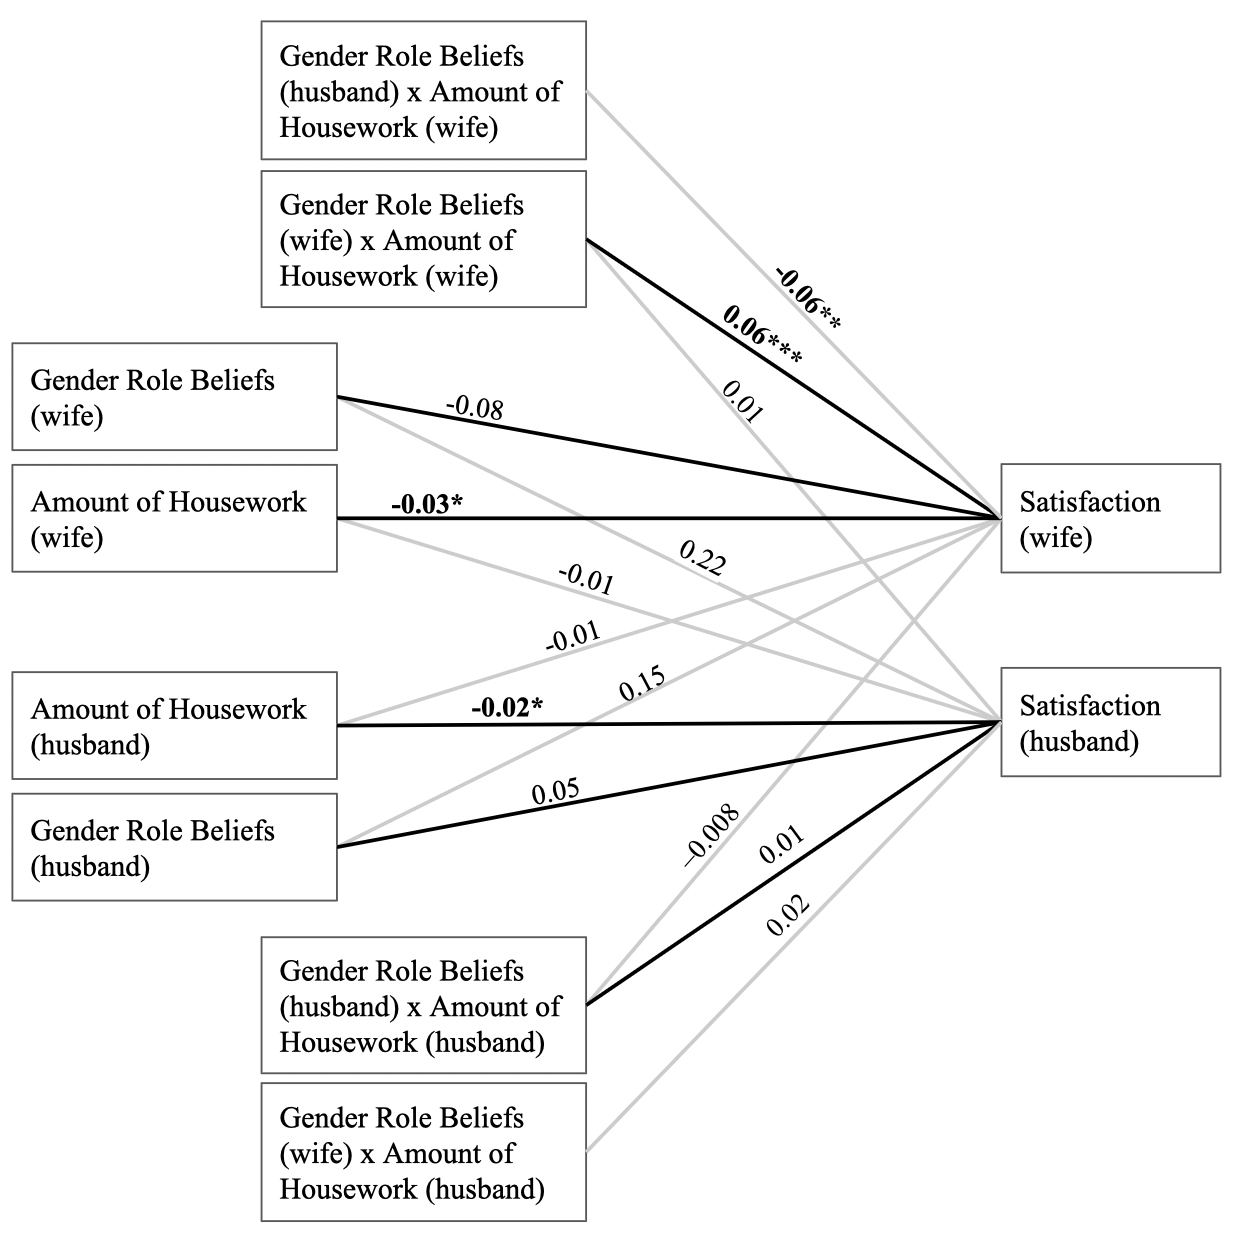
\includegraphics[width=4.25in]{moderation} \caption{Moderation effects in the APIM.}\label{fig:unnamed-chunk-8}
\end{figure}

Looking at the summary table above, these are the relationships that are statistically significant:
as.factor(genderE\_A)1:Cavg\_housework\_female\_A:Cavg\_grbs\_P, 8.742833e-03
as.factor(genderE\_A)1:Cavg\_housework\_female\_A:Cavg\_grbs\_A, 8.408625e-04
as.factor(genderE\_A)0:Cavg\_housework\_female\_A, 2.259373e-02

Only looking at the three way interactions with gender we found two significant gender differences in the moderation effects. The interaction between actors housework distribution and their own gender role beliefs was significantly different for husbands and wives with an estimate of 0.06 (\emph{p}=0.03,\emph{se}=0.03). The moderation effect of ones own gender role beliefs was 0.06 units higher for women than men meaning the moderation effect of gender role beliefs had a significantly larger positive effect on satisfaction for wives than for husbands.

In addition the interaction between actors housework distribution and their partners gender role beliefs was significantly different for husbands and wives with an estimate of -0.08(\emph{p}=0.01,\emph{se} = 0.03).The moderation effect of ones partners gender role beliefs was -0.08 units lower for women than men meaning the moderation effect of her husbands gender role beliefs had a significantly larger negative effect on satisfaction compared to how her gender role beliefs effected the relationship between housework distribution and satisfaction for her husband.

\begin{verbatim}
wife_plot<- ggplot(wives,aes(
                x = avg_housework_female_A,
                y = housework_satisfied_A, 
                color = grbs_hl_A,  na.rm = TRUE)
                )+
  geom_point(na.rm = TRUE)+
  geom_smooth(method = "lm")+
  labs(x = "Housework distribution", y = "Satisfaction", title ="Relationship of wive's housework distribution and gender role beliefs")
\end{verbatim}



\begin{verbatim}
## $title
## [1] "Relationship of wive's housework distribution and gender role beliefs"
## 
## attr(,"class")
## [1] "labels"
\end{verbatim}

\begin{figure}
\centering
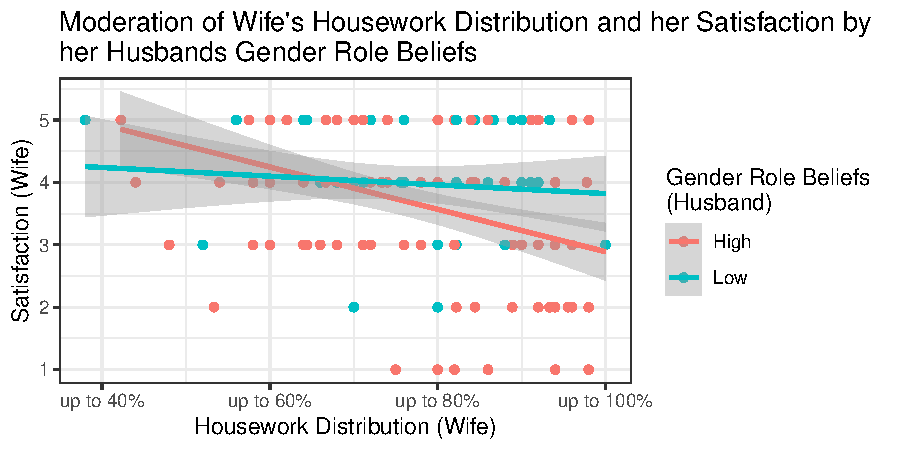
\includegraphics{results_files/figure-latex/unnamed-chunk-12-1.pdf}
\caption{\label{fig:unnamed-chunk-12}caption for graph}
\end{figure}



As the housework distribution increases for wives with low gender role beliefs, their satisfaction decreases. This makes sense because wives with low gender role beliefs would believe in an equal housework distribution where she wasn't doing majority of the housework tasks. As the housework distribution increases for wives with high gender role beliefs, their satisfaction has a very slight decrease, but it stays more or less the same.

\begin{figure}
\centering
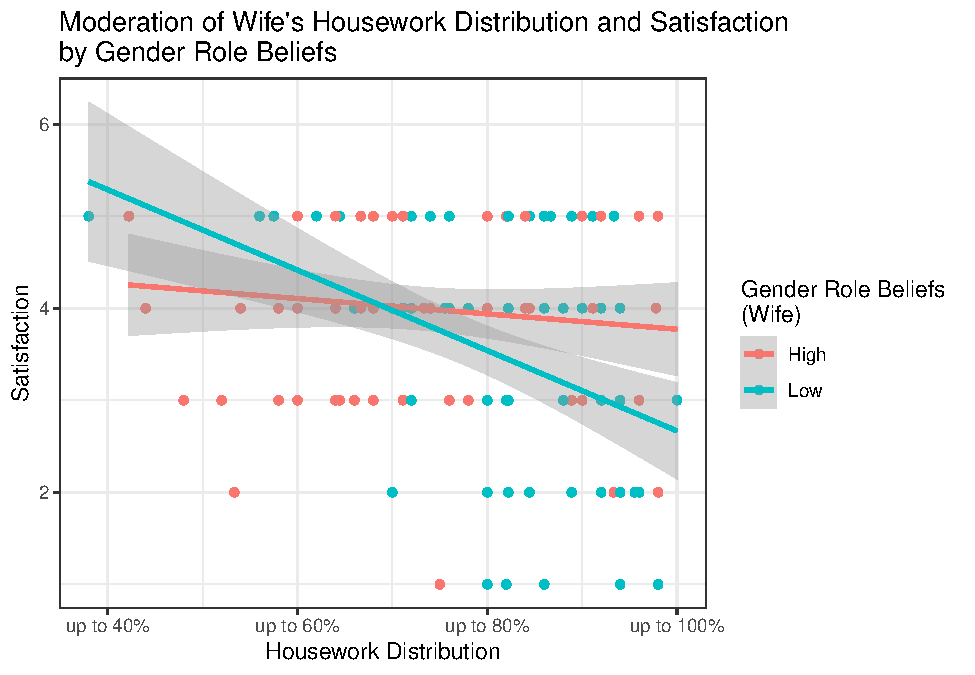
\includegraphics{results_files/figure-latex/unnamed-chunk-14-1.pdf}
\caption{\label{fig:unnamed-chunk-14}caption for graph}
\end{figure}

As the housework distribution increases for wives whose husbands have low gender role beliefs, their satisfaction remains constant. As the housework distribution increases for wives whose husbands have high gender role beliefs, their satisfaction decreases.

\hypertarget{religion}{%
\subsubsection{Religion}\label{religion}}

The two intercept model gives us the two coefficients for men and women.

None of the interactions between actors housework distribution and their religion was significantly different for husbands or wives. (\emph{p}\textgreater=0.19,\emph{se}=0.08). None of the results illustrate that the average female-typed tasks completed by the actor or partner from the husband and wife's perspective was related to their religion.

\hypertarget{exploratory-results}{%
\subsection{Exploratory Results}\label{exploratory-results}}

Mediation is a way for researchers to explain the process of one variable affecting another variable. It is essentially a possible explanation for the relationship between the two variables. Mediation assesses whether the effects of the X variable (the independent variable) are significant on the Y variable (the dependent variable), through a third variable called M (the mediator).

Based on our primary analysis so far, we are interested in further exploring how to concept of gatekeeping fits into our research. We want to explore whether gatekeeping is a mediator variable in our relationship between the partners' gender role beliefs and housework tasks. Are women with higher gender role beliefs more likely to gatekeep housework tasks?

\hypertarget{interpretation}{%
\paragraph{Interpretation:}\label{interpretation}}

All four paths are positive and statistically significant: Seeing your partner positively leads you and your partner to be more satisfied. All four of these paths could potentially be mediated.

\#\#\#Step 2: Testing the effects of the grbs (X) on the mediators of Wife and Husband gatekeeping (M).

\hypertarget{interpretation-1}{%
\paragraph{Interpretation:}\label{interpretation-1}}

All four paths of the ``a'' paths are negative and statistically significant: Seeing your partner positively leads you and your partner to have lower levels of tension.

\hypertarget{steps-3-and-4-testing-the-effects-of-the-tension-m-and-other-positivity-x-on-the-satisfaction-y.}{%
\subsubsection{Steps 3 and 4: Testing the effects of the Tension (M) and Other Positivity (X) on the Satisfaction (Y).}\label{steps-3-and-4-testing-the-effects-of-the-tension-m-and-other-positivity-x-on-the-satisfaction-y.}}

\hypertarget{i-didnt-change-anything-from-here-on-yet}{%
\paragraph{I didn't change anything from here on yet!}\label{i-didnt-change-anything-from-here-on-yet}}

\hypertarget{interpretation-2}{%
\paragraph{Interpretation:}\label{interpretation-2}}

\textbf{Step 3}: All four ``b'' paths from Tension to Satisfaction are negative and three are statistically significant: Seeing more tension in the relationship leads to less satisfaction for you and your partner, even after controlling for how positively you and your partner see each other. The one effect that is not statistically significant is the effect of male's level of tension on his wife's level of satisfaction.\\
\textbf{Step 4}: All paths from Other Positivity to Satisfaction, the direct of c', are positive and statistically significant: Seeing your partner positively leads you and your partner to have higher levels of satisfaction, even after controlling for yours and your partner's tension.

\hypertarget{testing-indirect-effects-using-multilevel-modeling}{%
\section{Testing Indirect Effects Using Multilevel Modeling}\label{testing-indirect-effects-using-multilevel-modeling}}

\begin{itemize}
\tightlist
\item
  Sobel Test

  \begin{itemize}
  \tightlist
  \item
    Save effect estimates and standard errors.
  \item
    Compute Z test.
  \item
    Low power.
  \end{itemize}
\item
  Separately Test a and b

  \begin{itemize}
  \tightlist
  \item
    Old fashioned.
  \item
    But may be making a comeback.
  \end{itemize}
\item
  Bootstrapping

  \begin{itemize}
  \tightlist
  \item
    Difficult currently
  \item
    See Pituch \& Stapleton (Multivariate Behavioral Research, 2008) for a discussion of how to bootstrap in MLM.
  \item
    Option available in some MLM programs. Only for effects but not indirect effects.
  \end{itemize}
\item
  Monte Carlo Method

  \begin{itemize}
  \tightlist
  \item
    Appears to be the method of choice for MLMeM
  \end{itemize}
\end{itemize}

\hypertarget{sobel-test}{%
\subsection{Sobel Test}\label{sobel-test}}

\hypertarget{mcmam-selig-preacher-2008}{%
\subsection{\texorpdfstring{MCMAM \href{http://www.quantpsy.org/medmc/medmc.htm}{Selig \& Preacher, 2008}}{MCMAM Selig \& Preacher, 2008}}\label{mcmam-selig-preacher-2008}}

\begin{verbatim}
# Function that returns mcmc CI. 
# mcmamCI <- function(aval, bval, varA, varB, n){

# code (Selig & Preacher, 2008).
  #require(MASS)
  
  a=aval
  b=bval
  rep=n
  conf=95
  pest=c(a,b)
  acov <- matrix(c(varA, 0, 0, varB),2,2)

  mcmc <- mvrnorm(rep,pest,acov,empirical=FALSE)

  ab <- mcmc[,1]*mcmc[,2]

  low=(1-conf/100)/2
  upp=((1-conf/100)/2)+(conf/100)

  LL=quantile(ab,low)
  UL=quantile(ab,upp)
  LL=format(LL,digits=3)
  UL=format(UL,digits=3)

  CI <- cbind.data.frame(LL, UL)
  return(CI)

\end{verbatim}

For example, we can find the MCMC 95\% CI for the \textbf{Actor-Actor: Husband} indirect effect like this.

act\_H\_a \textless- coef(summary(apim\_stp2)){[}3,1{]}
act\_H\_a\_se \textless- coef(summary(apim\_stp2)){[}3,2{]}
act\_H\_b \textless- coef(summary(apim\_stp3)){[}7,1{]}
act\_H\_b\_se \textless- coef(summary(apim\_stp3)){[}7,2{]}

mcmamCI(act\_H\_a, act\_H\_b, act\_H\_a\_se\^{}2, act\_H\_b\_se\^{}2, 3000)
\#confidence intervals \textgreater{} does it include 0?

```

\hypertarget{summary-of-indirect-effects}{%
\subsection{Summary of Indirect Effects}\label{summary-of-indirect-effects}}

\begin{longtable}[]{@{}cccccc@{}}
\toprule
Name & Indirect Effects & Estim. & p & 95\% CI\textsuperscript{a} Lower & Upper \\
\midrule
\endhead
Actor-Actor: W & Xw -\textgreater{} Mw -\textgreater{} Yw & 0.165 & \textless.001 & 0.086 & 0.257 \\
Actor-Actor: H & Xh -\textgreater{} Mh -\textgreater{} Yh & 0.099 & \textless.001 & 0.042 & 0.172 \\
Partner-Partner: W & Xw -\textgreater{} Mh -\textgreater{} Yw & 0.027 & .090 & -0.003 & 0.070 \\
Partner-Partner: H & Xh -\textgreater{} Mw -\textgreater{} Yh & 0.034 & .024 & 0.003 & 0.079 \\
Actor-Partner: W & Xh -\textgreater{} Mh -\textgreater{} Yw & 0.038 & .086 & -0.005 & 0.092 \\
Actor-Partner: H & Xw -\textgreater{} Mw -\textgreater{} Yh & 0.060 & .004 & 0.017 & 0.115 \\
Partner-Actor: W & Xh -\textgreater{} Mw -\textgreater{} Yw & 0.094 & .023 & 0.013 & 0.186 \\
Partner-Actor: H & Xw -\textgreater{} Mh -\textgreater{} Yh & 0.072 & .003 & 0.023 & 0.134 \\
\bottomrule
\end{longtable}

\textsuperscript{a}Bootstrapped CI using MCM
(The above table was produced by an Excel spreadsheet: IndirectEffects.xls.)

\hypertarget{summary-direct-and-total-effects}{%
\subsection{Summary Direct and Total Effects}\label{summary-direct-and-total-effects}}

\begin{longtable}[]{@{}cccccc@{}}
\toprule
Name & Direct Effects & Direct & p & Total\textsuperscript{a} & \% Mediated \\
\midrule
\endhead
Actor: Wife & Xw -\textgreater{} Yw & 0.185 & .007 & 0.378 & 50.9 \\
Actor: Husband & Xh -\textgreater{} Yh & 0.291 & \textless.001 & 0.424 & 31.5 \\
Partner: Wife & Xh -\textgreater{} Yw & 0.190 & .010 & 0.321 & 40.9 \\
Partner: Husband & Xw -\textgreater{} Yh & 0.129 & .028 & 0.262 & 50.8 \\
\bottomrule
\end{longtable}

\textsuperscript{a}Computed as \texttt{ab\ +\ c\textquotesingle{}} and \texttt{c} with results agreeing.

Note that \texttt{\%\ Mediated} equals \texttt{ab/c} or equivalently \texttt{1\ -\ c\textquotesingle{}/c}. This value can be larger than one or negative. First, make sure that \texttt{c} is substantial. If it is, then if \texttt{\%\ Mediated} is greater than 100 or negative, you have ``inconsistent mediation'': the direct and indirect effects are of opposite signs.


\clearpage
\renewcommand{\listfigurename}{Figure captions}

\clearpage
\renewcommand{\listtablename}{Table captions}


\end{document}
